% Generated by mml_research.motion.make_benchmark_tables.
% Needs \usepackage{booktabs,adjustbox,graphicx}.

\begin{figure}[ht]
\centering
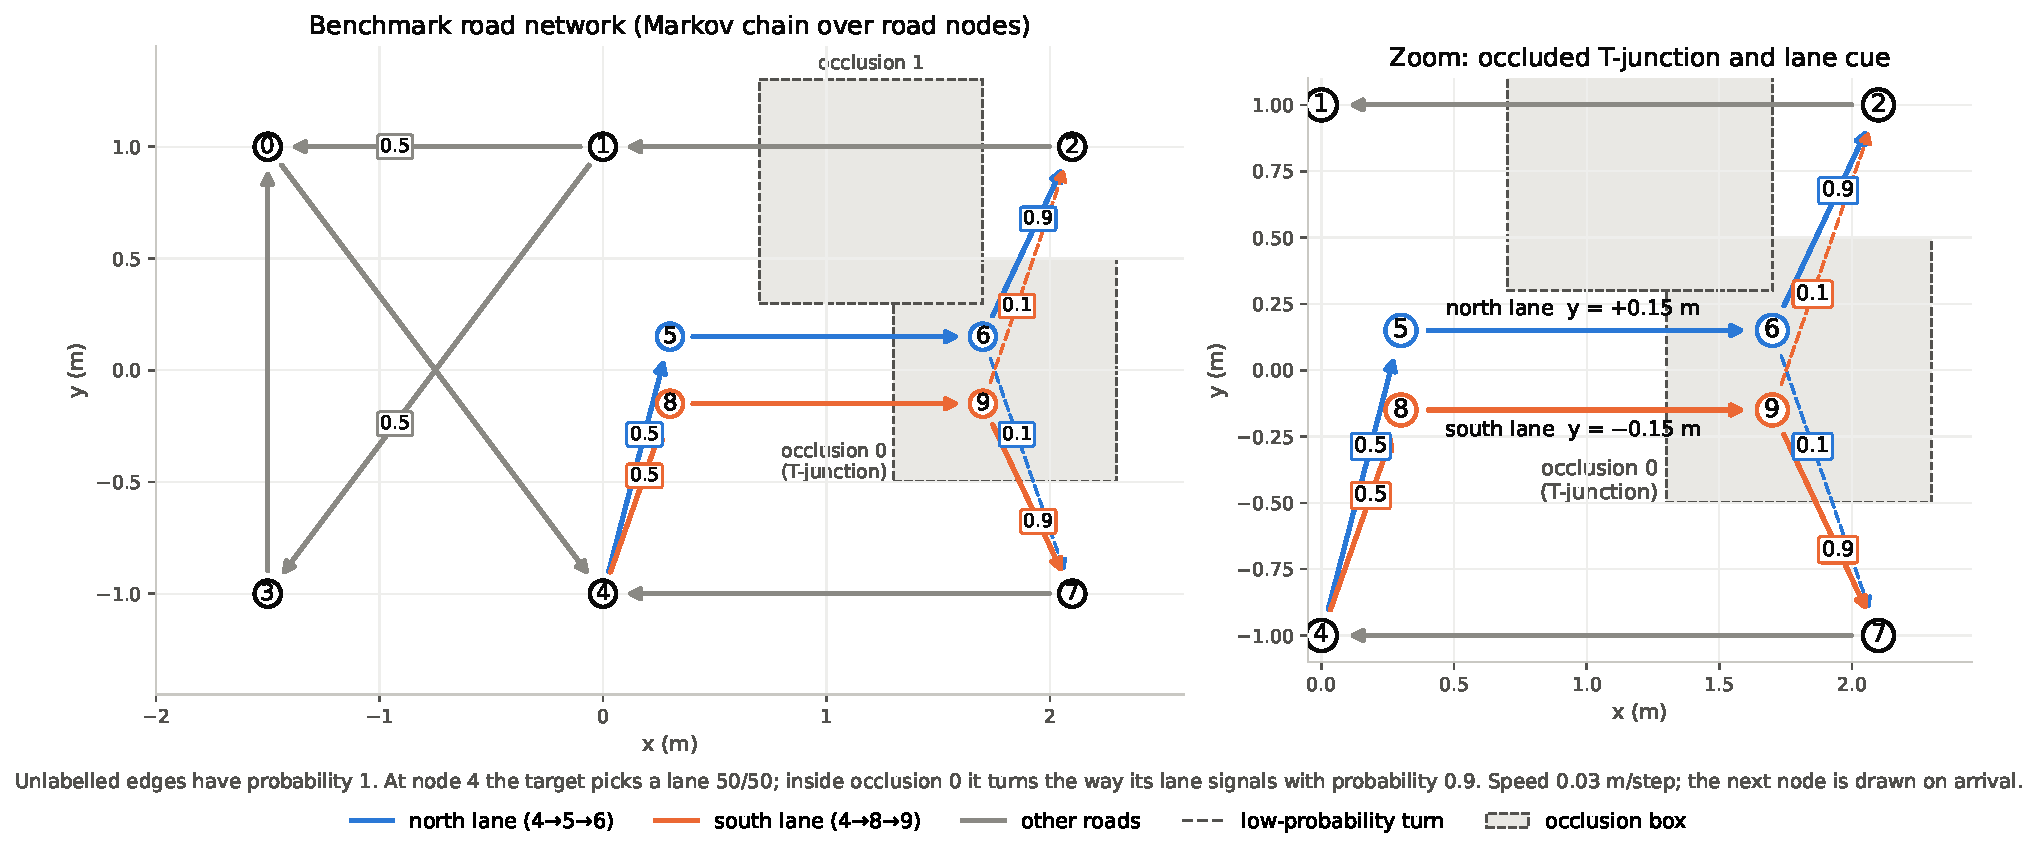
\includegraphics[width=\linewidth]{road_network.pdf}
\caption{Benchmark road network as a Markov chain over road nodes (positions in metres). The target drives the edges at 0.03\,m per step and draws its next node on arrival; unlabelled edges have probability 1. At node 4 it picks the north lane (4$\to$5$\to$6, $y{=}{+}0.15$\,m) or the south lane (4$\to$8$\to$9, $y{=}{-}0.15$\,m) with probability 0.5 each. The T-junction (nodes 6 and 9) lies inside occlusion 0, so the turn happens while the target is hidden; it turns the way its lane signals with probability 0.9. These junction occlusions are the 701 exit-prediction events of Tables~\ref{tab:exit-benchmark-tuned} and~\ref{tab:exit-benchmark-shared}, where the lane cue predicts the exit in 638 (91.0\%). Node 1 is a visible 50/50 junction; occlusion 1 covers a straight road with a single exit and is not scored. Right: zoom on the occluded T-junction.}
\label{fig:road-network}
\end{figure}

\begin{table}[ht]
\centering
\small
\caption{Filter-level tracking and exit-prediction benchmark with per-tracker process noise (lower RMSE and runtime, higher exit metrics are better). 100 seeded runs of 2000 steps (runs 0--99), identical trajectories, measurement noise and filter seeds for every tracker; 500 particles per filter. Exit metrics are pooled over the 701 junction occlusions (occlusion box with two possible exits; Fig.~\ref{fig:road-network}). Mean $\pm$ 95\% CI: $t$-interval over runs for RMSE and runtime; run-level bootstrap for exit metrics.}
\label{tab:exit-benchmark-tuned}
\begin{adjustbox}{max width=\linewidth}
\begin{tabular}{lcccccccc}
\toprule
Tracker & Noise (m) & RMSE all (m) & RMSE visible (m) & RMSE occluded (m) & Exit top-1 (\%) & Exit $>$50\% (\%) & $P$(correct exit) & Runtime (ms/step) \\
\midrule
PF+CFM (fixed $\sigma{=}1.0$) & $0.045$ & $0.0742\pm0.00323$ & $0.0192\pm7.98\times10^{-5}$ & $0.182\pm0.00774$ & $45.5\pm3.7$ & $45.5\pm3.7$ & $0.421\pm0.0133$ & $24\pm1.68$ \\
PF+CFM-AS (adaptive $\sigma$) & $0.032$ & $0.0737\pm0.0032$ & $0.0196\pm2.05\times10^{-4}$ & $0.18\pm0.00773$ & $2.3\pm1.1$ & $2.1\pm1.0$ & $0.31\pm0.0103$ & $23.8\pm1.72$ \\
\midrule
PF+NF & $0.032$ & $\mathbf{0.0623\pm0.00515}$ & $\mathbf{0.0151\pm1.89\times10^{-4}}$ & $\mathbf{0.153\pm0.013}$ & $\mathbf{91.0\pm2.2}$ & $90.3\pm2.3$ & $0.661\pm0.0204$ & $21.9\pm1.4$ \\
DiffPF & -- & $0.355\pm0.00819$ & $0.24\pm0.00631$ & $0.703\pm0.0142$ & $45.2\pm3.8$ & $45.2\pm3.8$ & $0.452\pm0.0384$ & $2.47\pm0.287$ \\
PF+CV & $0.005$ & $0.0656\pm0.00215$ & $0.0261\pm2\times10^{-4}$ & $0.154\pm0.00549$ & $1.1\pm0.8$ & $0.0\pm0.0$ & $0.219\pm0.00343$ & $\mathbf{0.126\pm0.00965}$ \\
PF+DMMN & $0.045$ & $0.064\pm0.00629$ & $0.0186\pm8.87\times10^{-4}$ & $0.154\pm0.0158$ & $\mathbf{91.0\pm2.2}$ & $\mathbf{91.0\pm2.2}$ & $\mathbf{0.759\pm0.0182}$ & $11.9\pm0.839$ \\
\bottomrule
\end{tabular}
\end{adjustbox}
\par\smallskip\parbox{0.95\linewidth}{\footnotesize Process noise $q$ (per-step position jitter, m) chosen for each particle filter by lowest RMSE all on separate validation runs 100--119 (Table~\ref{tab:noise-sweep-rmse}); DiffPF uses its built-in propagation noise. Exit top-1: the side of the box holding the largest share of particle mass, predicting without measurements until 10 steps after the target re-appears, is the side the target exits through; Exit $>$50\%: more than half the mass is beyond that side; $P$(correct exit): mean mass beyond that side. The approach-lane cue predicts the exit in 638/701 (91.0\%) events, the best achievable exit success; chance is 50\%. Runtime measured with 20 benchmark processes sharing the CPU, so it is comparable within this table only. Bold marks the best mean per column, not a statistically significant difference.}
\end{table}

\begin{table}[ht]
\centering
\small
\caption{Same benchmark with one shared process noise $q{=}0.01$\,m for every particle filter (lower RMSE and runtime, higher exit metrics are better). 100 seeded runs of 2000 steps (runs 0--99), identical trajectories, measurement noise and filter seeds for every tracker; 500 particles per filter. Exit metrics are pooled over the 701 junction occlusions (occlusion box with two possible exits; Fig.~\ref{fig:road-network}). Mean $\pm$ 95\% CI: $t$-interval over runs for RMSE and runtime; run-level bootstrap for exit metrics.}
\label{tab:exit-benchmark-shared}
\begin{adjustbox}{max width=\linewidth}
\begin{tabular}{lccccccc}
\toprule
Tracker & RMSE all (m) & RMSE visible (m) & RMSE occluded (m) & Exit top-1 (\%) & Exit $>$50\% (\%) & $P$(correct exit) & Runtime (ms/step) \\
\midrule
PF+CFM (fixed $\sigma{=}1.0$) & $0.103\pm0.00668$ & $0.063\pm0.00694$ & $0.212\pm0.00883$ & $\mathbf{91.0\pm2.2}$ & $\mathbf{91.0\pm2.2}$ & $0.801\pm0.02$ & $17.8\pm0.768$ \\
PF+CFM-AS (adaptive $\sigma$) & $\mathbf{0.0823\pm0.0042}$ & $0.0394\pm0.003$ & $0.186\pm0.00814$ & $42.9\pm3.6$ & $42.8\pm3.6$ & $0.39\pm0.0125$ & $17.6\pm0.823$ \\
\midrule
PF+NF & $0.126\pm0.023$ & $0.105\pm0.0266$ & $\mathbf{0.163\pm0.0131}$ & $\mathbf{91.0\pm2.2}$ & $\mathbf{91.0\pm2.2}$ & $0.766\pm0.0223$ & $17\pm0.676$ \\
DiffPF & $0.355\pm0.00819$ & $0.24\pm0.00631$ & $0.703\pm0.0142$ & $45.2\pm3.8$ & $45.2\pm3.8$ & $0.452\pm0.0384$ & $1.95\pm0.191$ \\
PF+CV & $0.0905\pm0.00174$ & $\mathbf{0.0211\pm8.56\times10^{-5}}$ & $0.224\pm0.00372$ & $80.5\pm2.7$ & $0.0\pm0.0$ & $0.268\pm0.00295$ & $\mathbf{0.108\pm0.00682}$ \\
PF+DMMN & $0.674\pm0.0611$ & $0.709\pm0.0627$ & $0.37\pm0.0675$ & $81.9\pm5.2$ & $81.9\pm5.2$ & $\mathbf{0.819\pm0.0517}$ & $9.24\pm0.36$ \\
\bottomrule
\end{tabular}
\end{adjustbox}
\par\smallskip\parbox{0.95\linewidth}{\footnotesize PF+DMMN gives every particle the same velocity, so at $q{=}0.01$ the cloud cannot follow the target through the visible junction and loses track in most runs. Exit top-1: the side of the box holding the largest share of particle mass, predicting without measurements until 10 steps after the target re-appears, is the side the target exits through; Exit $>$50\%: more than half the mass is beyond that side; $P$(correct exit): mean mass beyond that side. The approach-lane cue predicts the exit in 638/701 (91.0\%) events, the best achievable exit success; chance is 50\%. Runtime measured with 12 benchmark processes sharing the CPU. Bold marks the best mean per column, not a statistically significant difference.}
\end{table}

\begin{table}[ht]
\centering
\small
\caption{Process-noise sweep on validation runs: RMSE over all steps (m, lower is better) for per-step process noise $q$ (m). 20 runs of 2000 steps (runs 100--119, disjoint from the benchmark runs); mean $\pm$ 95\% $t$-interval over runs.}
\label{tab:noise-sweep-rmse}
\begin{adjustbox}{max width=\linewidth}
\begin{tabular}{lcccccc}
\toprule
Tracker & $q{=}0.005$ & $q{=}0.01$ & $q{=}0.02$ & $q{=}0.032$ & $q{=}0.045$ & $q{=}0.07$ \\
\midrule
PF+CFM (fixed $\sigma{=}1.0$) & $0.12\pm0.0165$ & $0.111\pm0.0145$ & $0.094\pm0.0114$ & $0.0811\pm0.0085$ & $\mathbf{0.0779\pm0.00736}$ & $0.088\pm0.00446$ \\
PF+CFM-AS (adaptive $\sigma$) & $0.0914\pm0.00991$ & $0.087\pm0.00939$ & $0.0791\pm0.00811$ & $\mathbf{0.0769\pm0.00733}$ & $0.0801\pm0.00602$ & $0.0982\pm0.00384$ \\
PF+NF & $0.18\pm0.0841$ & $0.137\pm0.057$ & $0.0765\pm0.0175$ & $\mathbf{0.0673\pm0.0128}$ & $0.0707\pm0.0105$ & $0.0996\pm0.00553$ \\
PF+CV & $\mathbf{0.0658\pm0.00559}$ & $0.0928\pm0.00356$ & $0.154\pm0.005$ & $0.177\pm0.0057$ & $0.186\pm0.00575$ & $0.191\pm0.00599$ \\
PF+DMMN & $1.2\pm0.183$ & $0.695\pm0.112$ & $0.108\pm0.0342$ & $0.0812\pm0.0189$ & $\mathbf{0.0719\pm0.0153}$ & $0.0791\pm0.00939$ \\
\bottomrule
\end{tabular}
\end{adjustbox}
\par\smallskip\parbox{0.95\linewidth}{\footnotesize Bold marks the lowest mean per row: the selection rule, fixed before the sweep, takes it; those values are used in Table~\ref{tab:exit-benchmark-tuned}. DiffPF has no process-noise parameter and is not swept.}
\end{table}

\begin{table}[ht]
\centering
\small
\caption{Process-noise sweep on validation runs: exit success with more than half the particle mass beyond the actual exit side (\%, higher is better). Same runs as Table~\ref{tab:noise-sweep-rmse}; mean $\pm$ 95\% run-level bootstrap CI.}
\label{tab:noise-sweep-exit}
\begin{adjustbox}{max width=\linewidth}
\begin{tabular}{lcccccc}
\toprule
Tracker & $q{=}0.005$ & $q{=}0.01$ & $q{=}0.02$ & $q{=}0.032$ & $q{=}0.045$ & $q{=}0.07$ \\
\midrule
PF+CFM (fixed $\sigma{=}1.0$) & $\mathbf{88.1\pm4.5}$ & $\mathbf{88.1\pm4.5}$ & $\mathbf{88.1\pm4.5}$ & $65.9\pm6.8$ & $37.8\pm8.6$ & $0.0\pm0.0$ \\
PF+CFM-AS (adaptive $\sigma$) & $\mathbf{35.6\pm8.5}$ & $\mathbf{35.6\pm8.4}$ & $28.9\pm7.7$ & $0.7\pm1.4$ & $0.0\pm0.0$ & $0.0\pm0.0$ \\
PF+NF & $\mathbf{88.1\pm4.5}$ & $\mathbf{88.1\pm4.5}$ & $\mathbf{88.1\pm4.5}$ & $\mathbf{88.1\pm4.5}$ & $54.1\pm9.7$ & $50.4\pm9.9$ \\
PF+CV & $0.0\pm0.0$ & $0.0\pm0.0$ & $0.0\pm0.0$ & $0.0\pm0.0$ & $0.0\pm0.0$ & $0.0\pm0.0$ \\
PF+DMMN & $57.0\pm10.0$ & $83.0\pm8.4$ & $\mathbf{88.1\pm4.5}$ & $\mathbf{88.1\pm4.5}$ & $\mathbf{88.1\pm4.5}$ & $86.7\pm4.9$ \\
\bottomrule
\end{tabular}
\end{adjustbox}
\par\smallskip\parbox{0.95\linewidth}{\footnotesize Process noise is added on every step, including occluded ones, so a larger $q$ widens the forecast while the target is hidden; this was not used for selection. Bold marks the best mean per row, not a statistically significant difference.}
\end{table}

\begin{table}[ht]
\centering
\small
\caption{Process-noise sweep on validation runs: mean particle mass beyond the actual exit side, $P$(correct exit) (higher is better). Same runs as Table~\ref{tab:noise-sweep-rmse}; mean $\pm$ 95\% run-level bootstrap CI.}
\label{tab:noise-sweep-pcorrect}
\begin{adjustbox}{max width=\linewidth}
\begin{tabular}{lcccccc}
\toprule
Tracker & $q{=}0.005$ & $q{=}0.01$ & $q{=}0.02$ & $q{=}0.032$ & $q{=}0.045$ & $q{=}0.07$ \\
\midrule
PF+CFM (fixed $\sigma{=}1.0$) & $\mathbf{0.785\pm0.0401}$ & $0.766\pm0.0387$ & $0.694\pm0.035$ & $0.543\pm0.0308$ & $0.393\pm0.0282$ & $0.282\pm0.0198$ \\
PF+CFM-AS (adaptive $\sigma$) & $0.362\pm0.0257$ & $\mathbf{0.366\pm0.0257}$ & $0.345\pm0.0245$ & $0.287\pm0.0212$ & $0.237\pm0.0172$ & $0.225\pm0.0157$ \\
PF+NF & $\mathbf{0.768\pm0.0495}$ & $0.759\pm0.0511$ & $0.728\pm0.0528$ & $0.661\pm0.0487$ & $0.581\pm0.0419$ & $0.459\pm0.0309$ \\
PF+CV & $0.222\pm0.00583$ & $\mathbf{0.265\pm0.00585}$ & $0.219\pm0.00605$ & $0.194\pm0.00588$ & $0.191\pm0.00547$ & $0.203\pm0.0044$ \\
PF+DMMN & $0.568\pm0.1$ & $0.83\pm0.0836$ & $\mathbf{0.877\pm0.0452}$ & $0.832\pm0.0451$ & $0.748\pm0.0424$ & $0.579\pm0.0285$ \\
\bottomrule
\end{tabular}
\end{adjustbox}
\par\smallskip\parbox{0.95\linewidth}{\footnotesize Not used for selection. Bold marks the best mean per row, not a statistically significant difference.}
\end{table}
